% Provenance (never printed): enseignement scientifique premiere (2019),
% theme "La Terre, un astre singulier: la forme de la Terre" (Eratosthenes,
% meridian measurement by triangulation, the metre); see
% sources/book2/PROVENANCE.md. Every length on the ellipsoid is computed in
% figdata/grade-10/meridian_degree.py (WGS 84, ledger wgs84:ellipsoid).
\chapter{पृथ्वी को मापना}\label{ch:g10:measuring-the-earth}

किसी समुद्र तट पर खड़े होकर खुले समुद्र की ओर जाते किसी जहाज़ को देखिए। वह केवल छोटा
होते-होते आँखों से ओझल नहीं होता: पहले उसका पेंदा गायब होता है, मानो वह डूब रहा हो, फिर
उसके ऊपरी ढाँचे का निचला भाग, और सबसे अंत में उसके मस्तूल का सिरा। आपके और जहाज़ के बीच
का समुद्र समतल नहीं है; वह उभरा हुआ है। बाईस सदियों से भी पहले सिकंदरिया के एक विद्वान ने
ऐसे ही एक प्रेक्षण --- दोपहर की छाया की लंबाई --- को पूरे ग्रह के आकार के मापन में बदल
दिया। यह अध्याय उस मापन का और उसके बाद आए मापनों का अनुसरण करता है: त्रिभुजों की वे
शृंखलाएँ जिन्हें सर्वेक्षकों ने पूरे-पूरे देशों में फैलाया, वे अभियान जो यह जानने के लिए
आर्कटिक और भूमध्य रेखा पर भेजे गए कि पृथ्वी चपटी है या नहीं, मीटर का जन्म, और वे उपग्रह
जिनसे आज ग्रह को मापा जाता है।

\begin{omfigure}
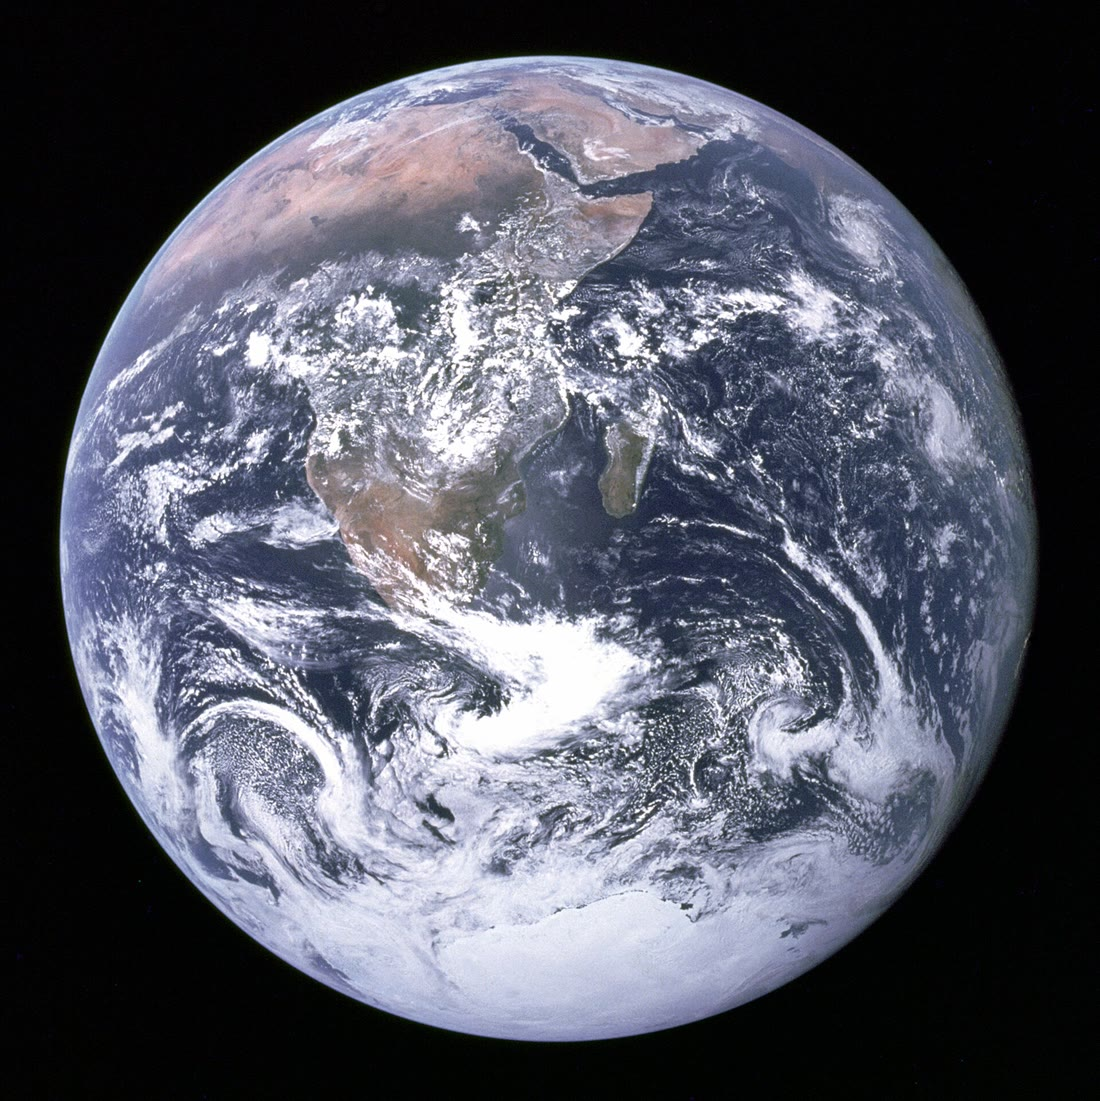
\includegraphics[width=0.5\linewidth]{images/book2/g10-nasa-apollo17-earth.jpg}

{\small अपोलो~17 के यात्रियों द्वारा दिसंबर 1972 में चंद्रमा की ओर जाते हुए खींची गई
पृथ्वी: अफ़्रीका, अरब और अंटार्कटिका की बर्फ़। फ़ोटो: NASA (सार्वजनिक
डोमेन)।}
\end{omfigure}

\begin{recall}
पृथ्वी पर किसी स्थान की स्थिति उसके अक्षांश से, यानी भूमध्य रेखा से उत्तर या दक्षिण में
उसके कोण से, और उसके देशांतर से, यानी किसी संदर्भ याम्योत्तर से पूर्व या पश्चिम में उसके
कोण से, बताई जाती है; याम्योत्तर ध्रुवों को जोड़ते हैं, और अक्षांश रेखाएँ भूमध्य रेखा के
समांतर पृथ्वी को घेरती हैं (पुस्तक 1)। एकसमान माध्यम में प्रकाश सीधी रेखाओं में चलता है,
और अत्यंत दूर स्थित सूर्य से पृथ्वी तक पहुँचने वाली किरणें समांतर होती हैं (भौतिकी की
पुस्तकें)। समकोण त्रिभुज में किसी न्यून कोण की ज्या सम्मुख भुजा को कर्ण से भाग देने पर,
उसकी कोज्या संलग्न भुजा को कर्ण से भाग देने पर, और उसकी स्पर्शज्या सम्मुख भुजा को संलग्न
भुजा से भाग देने पर मिलती है (गणित की पुस्तकें)।
\end{recall}

\section{गोल पृथ्वी}

अंतरिक्ष से पृथ्वी को देख पाने से बहुत पहले ही कई प्रेक्षणों ने दिखा दिया था कि वह गोल है।
\begin{itemize}
  \item \textbf{क्षितिज के पार जाते जहाज़।} दूर जाता जहाज़ नीचे से ऊपर की ओर ओझल होता है,
        हर दिशा में और हर समुद्र पर: समुद्र की सतह हर जगह वक्र है।
  \item \textbf{चंद्रमा पर छाया।} चंद्रग्रहण के समय पृथ्वी की छाया चंद्रमा पर पड़ती है। उसका
        किनारा हमेशा किसी वृत्त का चाप होता है, रात का समय चाहे जो हो; केवल गोला ही हर
        दिशा में गोल छाया डालता है।
  \item \textbf{अक्षांश के साथ तारे बदलते हैं।} उत्तर की ओर जाने वाला यात्री ध्रुव तारे को
        क्षितिज से ऊपर और ऊँचा चढ़ते देखता है, और दक्षिणी आकाश के तारे क्षितिज के नीचे
        छिप जाते हैं: वक्र सतह पर चलते हुए यात्री का क्षितिज झुकता जाता है।
  \item \textbf{पृथ्वी की परिक्रमा और अंतरिक्ष से दृश्य।} पहले जहाज़ों ने, फिर विमानों ने, हर
        दिशा में दुनिया का चक्कर लगाया है; 1960 के दशक से पूरे गोल ग्रह की फ़ोटो खींची
        जाती रही है।
\end{itemize}

\begin{omfigure}
\begin{tikzpicture}[font=\small, >={Stealth[length=2.2mm]}]
  % sea surface: arc of a circle of radius 8 centred at (0,-8) (curvature exaggerated)
  \fill[omDef!10] plot[domain=-4.6:4.6, samples=60] (\x,{sqrt(64-\x*\x)-8}) -- (4.6,-2.2) -- (-4.6,-2.2) -- cycle;
  \draw[omDef!70!black, thick] plot[domain=-4.6:4.6, samples=60] (\x,{sqrt(64-\x*\x)-8});
  % observer on a small tower at x=-4 (surface y=-1.072), eye at y=-0.235
  \draw[black!70, line width=1pt] (-4,-1.072) -- (-4,-0.235);
  \fill (-4,-0.235) circle (2pt);
  \node[anchor=east, align=right] at (-4.1,-0.2) {प्रेक्षक\\की आँख};
  % line of sight tangent at x=-0.5 (y=-0.0156, slope 0.0626)
  \draw[omThm!80!black, thick] (-4,-0.235) -- (4.4,0.290);
  \node[omThm!80!black, anchor=south, rotate=3.6] at (1.3,0.1) {दृष्टि रेखा};
  \fill[omThm!80!black] (-0.5,-0.0156) circle (1.4pt);
  % ship at x=3 (surface y=-0.584), tilted 22 degrees with the local vertical
  \begin{scope}[shift={(3,-0.584)}, rotate=-22]
    \fill[black!12] (-0.6,0) -- (0.6,0) -- (0.75,0.32) -- (-0.75,0.32) -- cycle;
    \draw[black!45, densely dashed] (-0.6,0) -- (0.6,0) -- (0.75,0.32) -- (-0.75,0.32) -- cycle;
    \draw[black!45, densely dashed] (0,0.32) -- (0,0.95);
    \draw[black!80, line width=1pt] (0,0.95) -- (0,1.55);
    \fill[black!80] (0,1.55) -- (0.32,1.25) -- (0,1.25) -- cycle;
  \end{scope}
  \node[anchor=north, align=center, font=\footnotesize] at (2.9,-1.25) {पेंदा और निचला मस्तूल\\उभार के पीछे छिपे};
  \node[anchor=north, font=\footnotesize] at (-0.5,-0.1) {क्षितिज};
\end{tikzpicture}

{\small जहाज़ नीचे से ऊपर की ओर क्यों ओझल होता है: प्रेक्षक को केवल वही दिखता है जो
क्षितिज पर समुद्र को छूती दृष्टि रेखा के ऊपर है। वक्रता बहुत बढ़ा-चढ़ाकर दिखाई गई है।}
\end{omfigure}

\section{एरातोस्थनीज़ पृथ्वी को मापते हैं}

साइरीन के एरातोस्थनीज़ (276--194 ईसा पूर्व) सिकंदरिया के पुस्तकालयाध्यक्ष थे। उन्होंने
सुना था कि नील नदी के बहुत ऊपर स्थित स्येने में, जो आज का असवान है, ग्रीष्म अयनांत के
दिन दोपहर को सूर्य एक कुएँ के पूरे तल को प्रकाशित कर देता था: तब वह ठीक सिर के ऊपर होता
था। उसी क्षण सिकंदरिया में एक ऊर्ध्वाधर छड़ी छोटी-सी छाया डालती थी: सूर्य की किरणें
ऊर्ध्वाधर से लगभग \qty{7.2}{\degree} का कोण बनाती थीं, जो पूरे वृत्त का पचासवाँ भाग है।
% ledger: erat:method, erat:stadion

\begin{omfigure}
\begin{tikzpicture}[font=\small, >={Stealth[length=2.2mm]}]
  \def\R{2.4}
  \fill[omDef!8] (0,0) circle (\R);
  \draw[omDef!70!black, thick] (0,0) circle (\R);
  \coordinate (O) at (0,0);
  \coordinate (S) at (\R,0);
  \coordinate (A) at ({\R*cos(25)},{\R*sin(25)});
  \coordinate (T) at ({(\R+0.75)*cos(25)},{(\R+0.75)*sin(25)});
  \coordinate (T2) at ({(\R+1.75)*cos(25)},{(\R+1.75)*sin(25)});
  % radii
  \draw[black!70] (O) -- (S);
  \draw[black!70] (O) -- (A);
  \draw[black!40, densely dashed] (A) -- (T2);
  \fill (O) circle (1.5pt) node[below left] {केंद्र};
  % stick at Alexandria, along the radius
  \draw[line width=1.6pt, black!85] (A) -- ($(A)!0.6!(T)$);
  % well at Syene
  \draw[black!80, thick] ({\R-0.38},-0.12) -- (\R,-0.12) ($(S)+(0,0.12)$) -- ({\R-0.38},0.12);
  % parallel sun rays coming from the right
  \foreach \y in {-1.6,-0.8,0.8,1.6} \draw[->, omThm!70, thick] (6.6,\y) -- (4.4,\y);
  \draw[->, omThm!85!black, thick] (6.6,0) -- (\R+0.05,0);
  \draw[->, omThm!85!black, thick] (6.6,{(\R+0.45)*sin(25)}) -- ({(\R+0.45)*cos(25)+0.03},{(\R+0.45)*sin(25)});
  \node[omThm!85!black, align=center, anchor=west] at (4.6,2.35) {सूर्य का प्रकाश:\\समांतर किरणें};
  % angles
  \draw[omExo!80!black, thick] (0.75,0) arc (0:25:0.75);
  \node[omExo!80!black] at (1.05,0.22) {$\alpha$};
  \coordinate (Q) at ($(A)!0.6!(T)$);
  \draw[omExo!80!black, thick] ($(Q)+(0.8,0)$) arc (0:25:0.8);
  \node[omExo!80!black] at ($(Q)+({1.08*cos(12.5)},{1.08*sin(12.5)})$) {$\alpha$};
  \node[anchor=east] at ($(A)+(-0.12,0.18)$) {सिकंदरिया};
  \node[anchor=north west] at ($(S)+(0.3,-0.12)$) {स्येने};
  \node[font=\footnotesize, anchor=north] at ($(O)!0.5!(S)+(0.2,-0.05)$) {};
  \draw[<->, black!60] ({(\R-0.3)*cos(3)},{(\R-0.3)*sin(3)}) arc (3:22:{\R-0.3});
  \node[anchor=east, font=\footnotesize] at ({(\R-0.35)*cos(13)},{(\R-0.35)*sin(13)}) {$d$};
\end{tikzpicture}

{\small एरातोस्थनीज़ का तर्क। स्येने में सूर्य सिर के ठीक ऊपर है: उसकी किरणें पृथ्वी के केंद्र
की ओर इंगित करती हैं। सिकंदरिया में एक ऊर्ध्वाधर छड़ी, जो स्वयं भी केंद्र की ओर इंगित करती
है, किरणों के साथ कोण $\alpha$ बनाती है। दोनों स्थानों के बीच केंद्र पर बना कोण भी यही
$\alpha$ है। कोण बढ़ाकर दिखाया गया है: वह केवल \qty{7.2}{\degree} था।}
\end{omfigure}

\begin{proposition}[एरातोस्थनीज़ का संबंध]\label{prop:g10:measuring-the-earth:eratosthenes}
यदि दो स्थान एक ही याम्योत्तर पर एक-दूसरे से दूरी $d$ पर हों, और दोपहर को सूर्य की
किरणें ऊर्ध्वाधर से जो कोण बनाती हैं उनमें $\alpha$ (अंशों में) का अंतर हो, तो पृथ्वी की
परिधि है
\[
  C = \frac{\qty{360}{\degree}}{\alpha}\, d .
\]
\end{proposition}

\begin{proof}
सूर्य इतनी दूर है कि दोनों स्थानों तक पहुँचने वाली उसकी किरणें समांतर हैं। हर स्थान पर
ऊर्ध्वाधर पृथ्वी के केंद्र की ओर इंगित करता है। चित्र में छड़ी तक पहुँचने वाली किरण और
स्येने से होकर जाने वाली त्रिज्या दो समांतर रेखाएँ हैं, और सिकंदरिया से होकर जाने वाली
त्रिज्या दोनों को काटती है: छड़ी और किरण के बीच का कोण
$\alpha$ और दोनों त्रिज्याओं के बीच केंद्र पर बना कोण एकांतर कोण हैं, इसलिए बराबर हैं।
चाप $d$ पूरी परिधि का उतना ही भाग है जितना कोण $\alpha$ एक पूरे
चक्कर का: $d/C = \alpha/\qty{360}{\degree}$।
\end{proof}

\begin{method}[दो छायाओं से परिधि मापना]\label{met:g10:measuring-the-earth:shadows}
\begin{enumerate}
  \item (लगभग) एक ही याम्योत्तर पर स्थित दो स्थान चुनिए और उनके बीच की उत्तर--दक्षिण
        दूरी $d$ मापिए।
  \item एक ही दिन स्थानीय दोपहर को हर स्थान पर एक ऊर्ध्वाधर छड़ी और सूर्य की किरणों के
        बीच का कोण मापिए: $\tan \theta = s/h$,
        जहाँ $h$ छड़ी की ऊँचाई है और $s$ उसकी छाया की लंबाई। सूर्य की ओर
        कभी मत देखिए: कोण केवल छाया से पढ़ा जाता है।
  \item दोनों कोणों का अंतर $\alpha$ लीजिए और
        $C = (360/\alpha)\,d$ लगाइए।
\end{enumerate}
\end{method}

\begin{example}[एरातोस्थनीज़ की संख्याएँ]\label{ex:g10:measuring-the-earth:numbers}
% ledger: erat:method, erat:stadion
एरातोस्थनीज़ ने सिकंदरिया से स्येने तक की दूरी 5000
\emph{स्टेडियन} मानी, जो लंबाई की एक यूनानी इकाई थी। $\alpha = 1/50$ वृत्त लेने पर,
\[
  C = 50 \times 5000 = 250\,000 \text{ स्टेडियन}.
\]
एक स्टेडियन कितना लंबा था? इतिहासकार आज भी इस पर बहस करते हैं।
\qty{157.2}{m} लेने पर $C \approx \qty{39300}{km}$; \qty{166.7}{m} लेने पर
$C \approx \qty{41700}{km}$। याम्योत्तर की वास्तविक परिधि
\qty{40008}{km} है: दोनों ही स्थितियों में एरातोस्थनीज़ कुछ ही प्रतिशत के भीतर सही थे।
\end{example}

\begin{remark}[क्या मान लिया गया था]\label{rem:g10:measuring-the-earth:assumptions}
एरातोस्थनीज़ ने गोलाकार पृथ्वी मानी, इतनी दूर स्थित सूर्य कि उसकी किरणें समांतर हों,
स्येने ठीक कर्क रेखा पर (जहाँ सूर्य सिर के ठीक ऊपर आ सकता है), और स्येने सिकंदरिया के ठीक
दक्षिण में। इनमें से हर बात लगभग सही थी, पर पूरी तरह नहीं: असवान सिकंदरिया से देशांतर में
लगभग \qty{3}{\degree} पूर्व में है। महत्व दूरी के उत्तर--दक्षिण भाग का है, यानी उस भाग का जो
याम्योत्तर के अनुदिश है।
% ledger: geonames:aswan, geonames:alexandria
\end{remark}

\section{त्रिभुजन}

ज़मीन पर किसी लंबी दूरी को ज़ंजीर या छड़ से मापना धीमा काम है, और नदियों, जंगलों और
पहाड़ों के आर-पार असंभव। दूसरी ओर, कोण बहुत सटीकता से मापे जा सकते हैं: एक अंशांकित
वृत्त पर लगी दूरबीन को बारी-बारी से दो दूर के संकेतों की ओर घुमाकर। अठारहवीं सदी से
सर्वेक्षकों ने इसी से पूरे-पूरे देश मापे।

\begin{definition}[भूगणित]\label{def:g10:measuring-the-earth:geodesy}
\emph{भूगणित}\index{भूगणित} वह विज्ञान है जो पृथ्वी की आकृति और आकार तथा उसकी सतह
पर बिंदुओं की स्थितियाँ मापता है, और यह देखता है कि वे समय के साथ कैसे
बदलती हैं।
\end{definition}

\begin{definition}[त्रिभुजन]\label{def:g10:measuring-the-earth:triangulation}
\emph{त्रिभुजन}\index{त्रिभुजन} त्रिभुजों की एक शृंखला द्वारा दूर के बिंदुओं की स्थिति
ज्ञात करता है: एक भुजा, \emph{आधार रेखा}, ज़मीन पर बड़ी सावधानी से मापी जाती है;
त्रिभुजों के सभी कोण उनके शीर्षों से मापे जाते हैं; फिर बाक़ी हर भुजा परिकलित की
जाती है।
\end{definition}

यह परिकलन किसी भी त्रिभुज की भुजाओं और कोणों के बीच के एक संबंध पर टिका है। त्रिभुज
$ABC$ में $a$, $b$, $c$ से शीर्षों $A$, $B$, $C$ की सम्मुख भुजाएँ दर्शाइए, और
$A$, $B$, $C$ से इन्हीं शीर्षों पर बने कोण भी।

\begin{proposition}[ज्या नियम]\label{prop:g10:measuring-the-earth:sine-rule}
किसी भी त्रिभुज $ABC$ में,
\[
  \frac{a}{\sin A} = \frac{b}{\sin B} = \frac{c}{\sin C}.
\]
\end{proposition}

\begin{proof}
$C$ से ऊँचाई खींचिए, जो रेखा $AB$ से $H$ पर मिलती है (नीचे के चित्र का दूसरा भाग);
$h = CH$ लिखिए। समकोण त्रिभुज $AHC$ में $\sin A = h/b$,
इसलिए $h = b \sin A$। समकोण त्रिभुज $BHC$ में $\sin B = h/a$, इसलिए
$h = a \sin B$। अतः $b \sin A = a \sin B$, यानी $a/\sin A = b/\sin B$।
(यदि $B$ पर का कोण अधिक कोण हो, तो $H$ बिंदु $B$ के आगे पड़ता है और $B$ पर समकोण
त्रिभुज का कोण $\qty{180}{\degree} - B$ होता है, जिसकी ज्या वही है।)
$A$ से खींची ऊँचाई के साथ यही तर्क $b/\sin B = c/\sin C$ देता है।
\end{proof}

\begin{omfigure}
\begin{tikzpicture}[font=\small, >={Stealth[length=2mm]}]
  \begin{scope}
    \coordinate (A) at (0,0); \coordinate (B) at (2.0,0.25);
    \coordinate (C) at (0.9,1.9); \coordinate (D) at (3.0,2.1);
    \coordinate (E) at (1.9,3.8); \coordinate (F) at (3.9,4.1);
    \coordinate (G) at (2.7,5.6);
    \draw[black!60] (A) -- (C) -- (B) (C) -- (D) -- (B) (C) -- (E) -- (D) -- (F) -- (E) -- (G) -- (F);
    \draw[omThm!85!black, line width=2pt] (A) -- (B);
    \foreach \p in {A,B,C,D,E,F,G} \fill (\p) circle (1.6pt);
    \node[below left] at (A) {$A$}; \node[below right] at (B) {$B$};
    \node[left] at (C) {$C$}; \node[right] at (D) {$D$};
    \node[left] at (E) {$E$}; \node[right] at (F) {$F$}; \node[above] at (G) {$G$};
    \node[omThm!85!black, anchor=north, font=\footnotesize] at (1.25,-0.3) {मापी गई आधार रेखा};
    \draw[omExo!80!black] ($(A)!0.28!(B)$) arc[start angle=7, end angle=64.6, radius=0.56];
    \draw[omExo!80!black] ($(B)!0.3!(A)$) arc[start angle=187, end angle=123, radius=0.6];
    \draw[black!50, densely dashed] (-0.5,0) -- (-0.5,5.6);
    \draw[->, black!70] (-0.5,5.0) -- (-0.5,5.8) node[above] {उ};
    \node[rotate=90, font=\footnotesize, black!60, anchor=south] at (-0.5,2.6) {याम्योत्तर};
  \end{scope}
  \begin{scope}[xshift=6.2cm, yshift=0.6cm]
    \coordinate (A) at (0,0); \coordinate (B) at (4,0); \coordinate (C) at (1.4,2.6);
    \coordinate (H) at (1.4,0);
    \draw[thick] (A) -- (B) -- (C) -- cycle;
    \draw[omDef!80!black, densely dashed] (C) -- (H);
    \draw[omDef!80!black] (1.4,0.22) -- (1.62,0.22) -- (1.62,0);
    \node[below left] at (A) {$A$}; \node[below right] at (B) {$B$};
    \node[above] at (C) {$C$}; \node[below] at (H) {$H$};
    \node[omDef!80!black, anchor=west] at (1.4,1.05) {$h$};
    \node[anchor=south east] at (0.7,1.3) {$b$};
    \node[anchor=south west] at (2.75,1.35) {$a$};
    \node[anchor=north] at (2.7,-0.02) {$c$};
    \draw[omExo!80!black] (0.5,0) arc (0:61.7:0.5);
    \draw[omExo!80!black] (3.45,0) arc (180:135:0.55);
  \end{scope}
\end{tikzpicture}

{\small बाएँ: एक मापी गई आधार रेखा $AB$ से याम्योत्तर के अनुदिश फैली त्रिभुजों की
शृंखला; चाप उपकरण से मापे गए अनेक कोणों में से दो को दिखाते हैं। दाएँ: ऊँचाई $h$, जो $C$ से खींची गई
है, दो तरह से लिखी जाकर
ज्या नियम देती है।}
\end{omfigure}

\begin{method}[त्रिभुजन शृंखला का परिकलन]\label{met:g10:measuring-the-earth:chain}
\begin{enumerate}
  \item पहले त्रिभुज $ABC$ में आधार रेखा $c = AB$ और
        $A$ तथा $B$ पर के कोण मापे जाते हैं; तीसरा कोण
        $C = \qty{180}{\degree} - A - B$ है (और उसका मापन बाक़ी कोणों की
        जाँच करता है)।
  \item ज्या नियम बाक़ी दो भुजाएँ देता है:
        $b = AC = c \sin B / \sin C$ और $a = BC = c \sin A / \sin C$।
  \item परिकलित भुजा अगले त्रिभुज की ज्ञात भुजा बन जाती है, और इसी तरह पूरी
        शृंखला में आगे।
  \item अंत में, हर भुजा का उत्तर--दक्षिण भाग याम्योत्तर से उसके कोण की कोज्या से
        परिकलित किया जाता है, और इन भागों को जोड़ा जाता है।
\end{enumerate}
\end{method}

\begin{example}[एक त्रिभुज]\label{ex:g10:measuring-the-earth:triangle}
एक आधार रेखा $AB = \qty{8.000}{km}$ मापी जाती है; $A$ से संकेत $C$
$B$ की दिशा से \qty{70}{\degree} पर दिखता है, और $B$ से
$A$ की दिशा से \qty{60}{\degree} पर। तब $C = \qty{50}{\degree}$ और
\[
  AC = \frac{8.000 \times \sin 60^\circ}{\sin 50^\circ} = \frac{8.000 \times 0.8660}{0.7660}
  \approx \qty{9.044}{km}, \qquad
  BC = \frac{8.000 \times \sin 70^\circ}{\sin 50^\circ} \approx \qty{9.814}{km}.
\]
आधार रेखा के सिवा कोई दूरी पैदल नहीं नापी गई।
\end{example}

\begin{example}[मीटर का याम्योत्तर]\label{ex:g10:measuring-the-earth:meridian}
% ledger: metre:1791, metre:survey, geonames:dunkirk, geonames:barcelona (arc computed in figdata/grade-10/meridian_degree.py)
मार्च 1791 में मीटर को ध्रुव से भूमध्य रेखा तक किसी याम्योत्तर के अनुदिश दूरी के
एक करोड़वें भाग के रूप में परिभाषित किया गया। वह दूरी ज्ञात करने के लिए दो खगोलविदों,
ज़ाँ-बातीस्त देलांब्र और पिएर मेशैं, ने उत्तर सागर के तट पर स्थित डनकर्क से भूमध्य सागर के
तट पर स्थित बार्सिलोना तक के याम्योत्तर चाप को \omterm{def:g10:measuring-the-earth:triangulation}{त्रिभुजन} से मापा --- लगभग सात वर्षों का
काम, उत्तरी दो-तिहाई भाग में देलांब्र, दक्षिणी एक-तिहाई में मेशैं। दोनों नगरों के अक्षांशों में
\qty{9.646}{\degree} का अंतर है; आधुनिक दीर्घवृत्तज पर उनकी अक्षांश रेखाओं के बीच का चाप
\qty{1072.2}{km} लंबा है। किसी चाप की लंबाई और उसके अक्षांश-अंतर को जानने से एक अंश की
लंबाई मिलती है; फिर पृथ्वी की आकृति पूरा चौथाई याम्योत्तर देती है। नए मीटर के प्लैटिनम
मानक 1799 में बनाए गए और राष्ट्रीय अभिलेखागार में रखे गए।
\end{example}

\begin{history}[पुनरावर्ती वृत्त]
मीटर के याम्योत्तर के कोण एक \emph{पुनरावर्ती
वृत्त} से मापे गए, जो ज़ाँ-शार्ल दे बोर्दा का बनाया उपकरण था: एक अंशांकित वृत्त पर
दो दूरबीनें, जिन्हें बारी-बारी से दो संकेतों की ओर बार-बार घुमाया जाता था, ताकि अंशांकन
पढ़ने की त्रुटियाँ पुनरावृत्तियों की संख्या से विभाजित हो जाएँ।
\begin{center}
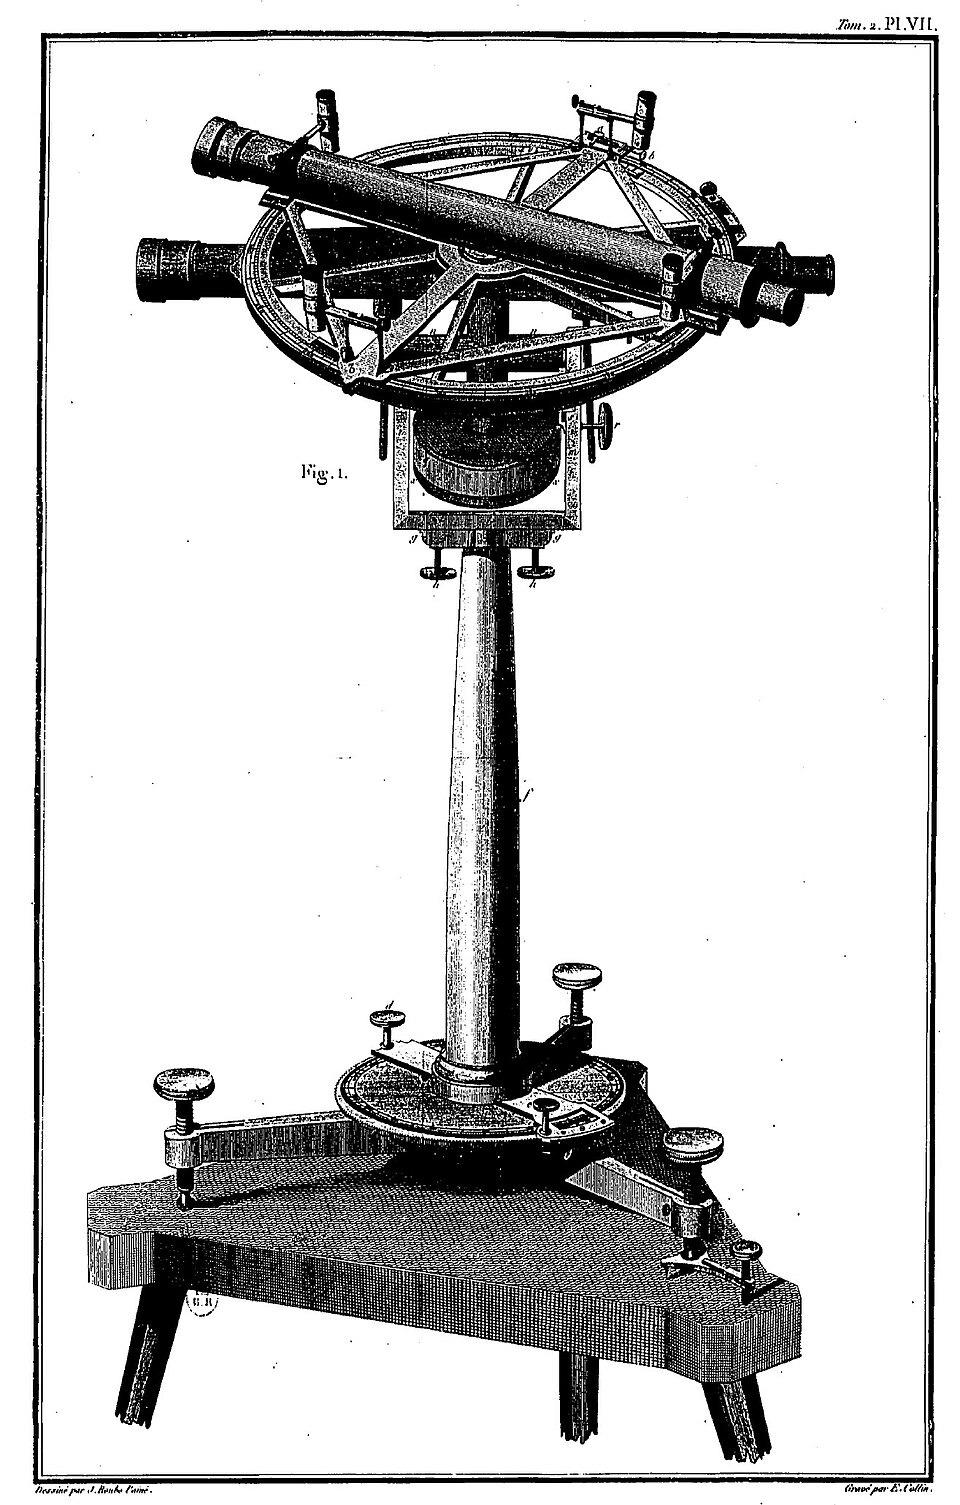
\includegraphics[width=0.3\linewidth]{images/book2/g10-delambre-repeating-circle.jpg}

{\small क्षैतिज कोण मापने के लिए लगाया गया एक पुनरावर्ती वृत्त, जैसा देलांब्र के मापन-विवरण
(1807) में उत्कीर्ण है। सार्वजनिक डोमेन (विकिमीडिया
कॉमन्स)।}
\end{center}
\end{history}

\section{चपटी पृथ्वी}

लगभग 1687 में आइज़क न्यूटन ने अपने गुरुत्वाकर्षण सिद्धांत से तर्क दिया कि घूमती पृथ्वी
ध्रुवों पर चपटा और भूमध्य रेखा पर उभरा हुआ एक गोलाभ होनी चाहिए। पेरिस वेधशाला के
खगोलविदों द्वारा किए गए याम्योत्तर के अंशों के मापन उलटी बात कहते लग रहे थे: ध्रुवों पर
खिंची हुई पृथ्वी। प्रश्न का निपटारा एक-दूसरे से यथासंभव दूर स्थानों पर अक्षांश के एक अंश
की लंबाई मापकर हुआ।
% ledger: figure:expeditions

\begin{omfigure}
\begin{tikzpicture}[font=\small, >={Stealth[length=2mm]}]
  \def\a{3.0} \def\b{2.3}
  \draw[black!35, densely dashed] (0,0) circle (\a);
  \fill[omDef!8] (0,0) ellipse ({\a} and {\b});
  \draw[omDef!70!black, thick] (0,0) ellipse ({\a} and {\b});
  \draw[black!50] (-3.4,0) -- (3.7,0);
  \draw[black!50] (0,-2.6) -- (0,3.3);
  \draw[<->, omThm!85!black] (0,-0.3) -- (\a,-0.3);
  \node[omThm!85!black, below] at (1.5,-0.3) {$a$};
  \draw[<->, omThm!85!black] (-0.3,0) -- (-0.3,\b);
  \node[omThm!85!black, left] at (-0.3,1.15) {$b$};
  \node[above right] at (0,\b) {उ};
  \node[anchor=south east] at (3.0,-2.5) {};
  \node[anchor=west] at (3.7,0) {भूमध्य रेखा};
  % normal at t = 45 deg: P = (2.121, 1.626); crosses the equator at (0.874,0), the axis at (0,-1.14)
  \coordinate (P) at (2.121,1.626);
  \draw[omExo!85!black, thick] (P) -- ($(P)!1.35!(0.874,0)$);
  \draw[omExo!85!black, thick, ->] (P) -- ($(P)!-0.45!(0.874,0)$);
  \fill (P) circle (1.6pt);
  \node[anchor=west, align=left, font=\footnotesize] at (2.85,2.35) {स्थानीय ऊर्ध्वाधर\\(साहुल)};
  \draw[omExo!85!black] (1.45,0) arc (0:52.5:0.58);
  \node[omExo!85!black] at (1.62,0.32) {$\varphi$};
  \fill (0,0) circle (1.3pt);
  \node[anchor=north east, font=\footnotesize] at (0,0) {केंद्र};
  \node[black!50, font=\footnotesize, anchor=south] at (-2.2,2.15) {गोला};
\end{tikzpicture}

{\small चपटी पृथ्वी, जिसका \omterm{def:g10:measuring-the-earth:ellipsoid}{चपटापन} बहुत बढ़ा-चढ़ाकर दिखाया गया है (वास्तविक \omterm{def:g10:measuring-the-earth:ellipsoid}{चपटापन}
इस पैमाने पर दिखने के लिए बहुत छोटा है)। किसी स्थान का ऊर्ध्वाधर सतह के लंबवत होता है;
वह ठीक केंद्र की ओर इंगित नहीं करता। स्थान का
अक्षांश $\varphi$ उसके ऊर्ध्वाधर और भूमध्य रेखा के तल के बीच का कोण है।}
\end{omfigure}

अक्षांश तारों से मापा जाता है: वह स्थानीय ऊर्ध्वाधर और भूमध्य रेखा के तल के बीच का कोण
है। चपटी पृथ्वी पर सतह भूमध्य रेखा के पास की तुलना में ध्रुवों के पास कम वक्र होती है।
जहाँ सतह कम वक्र हो, वहाँ ऊर्ध्वाधर को एक अंश घूमने के लिए सतह पर अधिक दूर चलना पड़ता
है: \emph{अक्षांश का एक अंश ध्रुवों के पास अधिक लंबा होता है}।

\begin{history}[लैपलैंड और पेरू]
% ledger: figure:expeditions, figure:degrees
1735 में पेरिस विज्ञान अकादमी ने एक अभियान भूमध्य रेखा पर, स्पेन के पेरू प्रांत में (आज का
इक्वाडोर), भेजा; उसने वहाँ नौ वर्ष, 1744 तक, काम किया। 1736--1737 में
पिएर-लुई मोरो दे मोपर्तुई के नेतृत्व में दूसरे अभियान ने, जिसमें युवा गणितज्ञ अलेक्सी क्लेरो
भी थे, आर्कटिक वृत्त के पास लैपलैंड में याम्योत्तर का एक अंश मापा। लैपलैंड का अंश
57\,437 \emph{तुआज़} (लंबाई की पुरानी इकाई; लगभग
\qty{111.95}{km}) निकला, और पेरू का अंश केवल 56\,737 तुआज़: अंश ध्रुव के पास अधिक
लंबा है, और न्यूटन सही थे। इन दो संख्याओं से लगभग $1/205$ का
\omterm{def:g10:measuring-the-earth:ellipsoid}{चपटापन} निकलता था --- बाद के सर्वेक्षणों के अनुसार बहुत अधिक, पर चिह्न का प्रश्न सुलझ
गया।
\end{history}

\begin{omfigure}
\begin{tikzpicture}
\begin{axis}[omrecord, width=0.82\linewidth, height=5.4cm, xmin=0, xmax=90,
  ymin=110.45, ymax=111.8, xlabel={अक्षांश (\unit{\degree})},
  ylabel={अक्षांश के \qty{1}{\degree} की लंबाई (km)}, xtick={0,15,...,90},
  ytick={110.6,110.8,...,111.8}, yticklabel style={/pgf/number format/fixed, /pgf/number format/fixed zerofill, /pgf/number format/precision=1}]
\addplot[omDef!85!black, line width=1.1pt] table[x=lat_deg, y=deg_km] {figdata/out/grade-10-meridian_degree.dat};
\addplot[only marks, mark=*, mark size=1.8pt, omThm!85!black] coordinates {(0,110.574) (45,111.132) (66,111.507) (90,111.694)};
\node[anchor=south west, font=\footnotesize] at (axis cs:2,110.6) {110.57 km};
\node[anchor=north east, font=\footnotesize] at (axis cs:89,111.56) {111.69 km};
\node[anchor=north west, font=\footnotesize] at (axis cs:46,111.12) {111.13 km};
\node[anchor=south east, font=\footnotesize] at (axis cs:65,111.53) {\ang{66} पर 111.51 km (लैपलैंड)};
\end{axis}
\end{tikzpicture}

{\small \omterm{def:g10:measuring-the-earth:ellipsoid}{संदर्भ दीर्घवृत्तज} (\cref{def:g10:measuring-the-earth:ellipsoid}) पर भूमध्य
रेखा से ध्रुव तक अक्षांश के एक अंश की लंबाई।
WGS~84 दीर्घवृत्तज से परिकलित।}
\end{omfigure}

\begin{definition}[संदर्भ दीर्घवृत्तज और चपटापन]\label{def:g10:measuring-the-earth:ellipsoid}
\emph{संदर्भ दीर्घवृत्तज}\index{संदर्भ दीर्घवृत्तज} वह सतह है जो किसी दीर्घवृत्त को
उसके लघु अक्ष के परितः घुमाने से मिलती है, और जिसे पृथ्वी की आकृति से यथासंभव निकटता से
मेल खाने के लिए चुना जाता है। उसकी \emph{विषुवतीय त्रिज्या}
$a$ है, उसकी \emph{ध्रुवीय त्रिज्या} $b$, और उसका
\emph{चपटापन}\index{चपटापन} है
\[
  f = \frac{a-b}{a}.
\]
\end{definition}

\begin{proposition}[पृथ्वी की विमाएँ]\label{prop:g10:measuring-the-earth:dimensions}
% ledger: wgs84:ellipsoid, earth:Req, earth:Rpol, earth:Rmean (lengths computed in figdata/grade-10/meridian_degree.py)
उपग्रह स्थिति-निर्धारण में प्रयुक्त \omterm{def:g10:measuring-the-earth:ellipsoid}{संदर्भ दीर्घवृत्तज} (WGS~84) के लिए
\[
  a = \qty{6378.137}{km}, \qquad b = \qty{6356.752}{km}, \qquad
  f = \frac{1}{298.257}.
\]
ध्रुवीय त्रिज्या विषुवतीय त्रिज्या से \qty{21.4}{km} छोटी है।
भूमध्य रेखा \qty{40075}{km} लंबी है और एक याम्योत्तर, ध्रुव से ध्रुव तक और वापस,
\qty{40008}{km}; चौथाई याम्योत्तर, भूमध्य रेखा से किसी ध्रुव तक,
\qty{10001.966}{km} है। अक्षांश का एक अंश भूमध्य रेखा पर \qty{110.574}{km} लंबा है
और ध्रुवों पर \qty{111.694}{km}। देशांतर का एक अंश भूमध्य रेखा पर
\qty{111.32}{km} लंबा है और ध्रुवों की ओर लगभग
$\cos \varphi$ के अनुसार घटता जाता है।
\end{proposition}

\begin{example}[देशांतर का एक अंश]\label{ex:g10:measuring-the-earth:longitude}
अक्षांश $\varphi$ पर स्थित अक्षांश रेखा एक वृत्त है जिसकी त्रिज्या अक्ष से दूरी है,
लगभग $R \cos \varphi$। \qty{60}{\degree} उत्तर पर उसकी
परिधि भूमध्य रेखा की परिधि की लगभग आधी है, और देशांतर का एक अंश
लगभग $111.32 \times \cos 60^\circ \approx \qty{55.7}{km}$ है
(दीर्घवृत्तज \qty{55.80}{km} देता है)।
\end{example}

\begin{remark}[गोल कितना गोल है?]\label{rem:g10:measuring-the-earth:round}
$1/298$ का \omterm{def:g10:measuring-the-earth:ellipsoid}{चपटापन} छोटा है। \qty{30}{cm} व्यास के ग्लोब पर ध्रुवीय
व्यास विषुवतीय व्यास से केवल \qty{1}{mm} छोटा होता ---
अदृश्य। सबसे गहरी महासागरीय खाई, समुद्र तल से लगभग \qty{11}{km} नीचे,
चौथाई मिलीमीटर गहरी एक खरोंच भर होती। अधिकांश कामों के लिए पृथ्वी
\qty{6371}{km} माध्य त्रिज्या का गोला है; सटीक स्थितियों के लिए दीर्घवृत्तज
आवश्यक है।
% ledger: earth:Rmean, usgs:trench-depth
\end{remark}

\section{आज का भूगणित}

\begin{omfigure}
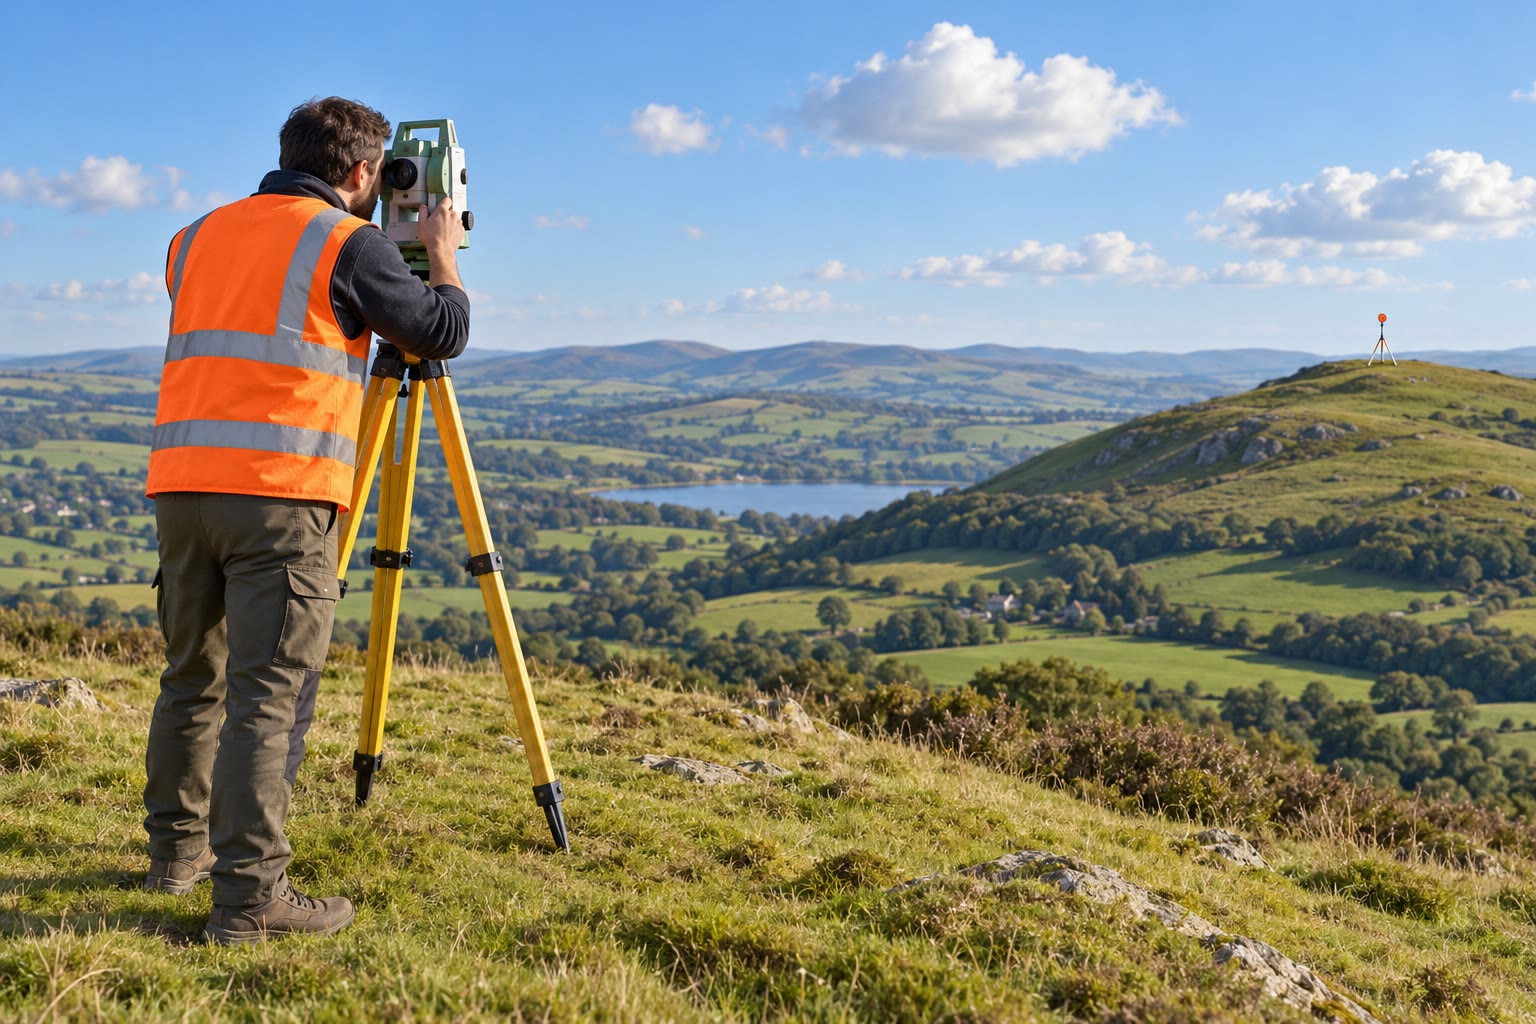
\includegraphics[width=0.7\linewidth]{images/book2/ai/g10-surveyor-theodolite.jpg}

{\small एक आधुनिक उपकरण के साथ काम करता सर्वेक्षक, जो कोण मापता है और प्रकाश की एक
किरण से दूरियाँ भी; दूर की पहाड़ी पर सर्वेक्षण का एक संकेत खड़ा
है।}
\end{omfigure}

अठारहवीं और उन्नीसवीं सदी के बड़े \omterm{def:g10:measuring-the-earth:triangulation}{त्रिभुजनों} की जगह अब उपग्रहों ने ले ली है। ज़मीन पर रखा
एक अभिग्राही कई ऐसे उपग्रहों के संकेत पकड़ता है जिनकी स्थितियाँ हर क्षण ज्ञात हैं, और
संकेतों के यात्रा-समय से अपनी स्थिति परिकलित करता है (पुस्तक 1)।
दुनिया भर में आधार-शैल पर स्थिर किए गए स्थायी अभिग्राहियों के जाल
लगातार अपनी स्थितियाँ मापते हैं। वे वह संदर्भ तंत्र परिभाषित करते हैं जिसमें
हर मानचित्र और हर उपग्रह-स्थिति दी जाती है, और वे खिसकते हैं: वे
स्थलमंडल की प्लेटों को कुछ सेंटीमीटर प्रति वर्ष की दर से खिसकते हुए दिखाते हैं
(\cref{ch:g11:plate-motions})।
% ledger: usgs:gps

\begin{inthefield}[आज ज़मीन को मापना]
भूगणितज्ञ इमारतों और पेड़ों से दूर, आधार-शैल में गड़े कंक्रीट के खंभों पर ऐंटेना लगाते हैं,
और वर्षों तक हर कुछ सेकंड पर उनकी स्थितियाँ दर्ज करते हैं।
वे इन्हें अत्यंत दूर की आकाशगंगाओं को देखने वाले रेडियो दूरबीनों के मापनों के साथ, और
दर्पण लगे उपग्रहों पर दागे गए लेज़र पुंजों के मापनों के साथ जोड़ते हैं।
निर्माण-स्थलों पर और ग्रामीण इलाक़ों में सर्वेक्षक आज भी तिपाइयों पर रखे उपकरणों से कोण और
दूरियाँ मापते हैं, और उन्हें उपग्रह-तंत्र से जोड़ते हैं।
\end{inthefield}

\section{अभ्यास}

\begin{exercise}[$\star$]\label{exo:g10:measuring-the-earth:1}
ज़मीन छोड़े बिना संभव ऐसे तीन प्रेक्षण बताइए जो दिखाते हैं कि पृथ्वी गोल है। हर एक के
लिए एक वाक्य में समझाइए कि समतल पृथ्वी उसे क्यों उत्पन्न नहीं कर
सकती।
\end{exercise}

\begin{exercise}[$\star$]\label{exo:g10:measuring-the-earth:2}
\omterm{def:g10:measuring-the-earth:geodesy}{भूगणित} क्या है? \omterm{def:g10:measuring-the-earth:triangulation}{त्रिभुजन} क्या है, और \omterm{def:g10:measuring-the-earth:triangulation}{त्रिभुजन} में ज़मीन पर केवल कौन-सी एक लंबाई
मापनी पड़ती है?
\end{exercise}

\begin{exercise}[$\star$]\label{exo:g10:measuring-the-earth:3}
एरातोस्थनीज़ ने पाया कि जब 5000 स्टेडियन दूर स्येने में सूर्य सिर के ठीक ऊपर था, तब
सिकंदरिया में सूर्य की किरणों और ऊर्ध्वाधर के बीच का कोण पूरे वृत्त का $1/50$ था।
परिधि पहले स्टेडियन में, फिर किलोमीटर में परिकलित कीजिए,
एक स्टेडियन को \qty{157.2}{m} मानकर।
\end{exercise}

\begin{exercise}[$\star$]\label{exo:g10:measuring-the-earth:4}
अक्षांश का एक अंश लगभग \qty{111}{km} लंबा है। अक्षांश का एक मिनट
($1/60$ अंश) कितना लंबा है? भूमध्य रेखा से ध्रुव तक का याम्योत्तर मोटे तौर पर कितना
लंबा है?
\end{exercise}

\begin{exercise}[$\star$]\label{exo:g10:measuring-the-earth:5}
विषुवतीय त्रिज्या \qty{6378.137}{km} और ध्रुवीय त्रिज्या
\qty{6356.752}{km} लेकर दोनों त्रिज्याओं का अंतर और
\omterm{def:g10:measuring-the-earth:ellipsoid}{चपटापन} $f = (a-b)/a$ परिकलित कीजिए। $f$ को एक बटा किसी पूर्ण संख्या के रूप में लिखिए।
\end{exercise}

\begin{exercise}[$\star\star$]\label{exo:g10:measuring-the-earth:6}
दो नगर एक ही याम्योत्तर पर \qty{500}{km} की दूरी पर हैं। एक ही दिन दोपहर को
\qty{1.00}{m} ऊँची एक ऊर्ध्वाधर छड़ी दक्षिणी नगर में \qty{0.364}{m} की और
उत्तरी नगर में \qty{0.456}{m} की छाया डालती है। हर नगर में सूर्य की किरणों और
ऊर्ध्वाधर के बीच का कोण परिकलित कीजिए, फिर पृथ्वी की
परिधि।
\end{exercise}

\begin{exercise}[$\star\star$]\label{exo:g10:measuring-the-earth:7}
त्रिभुज $ABC$ में आधार रेखा $AB = \qty{10.00}{km}$ है, $A$ पर का कोण
\qty{62}{\degree} और $B$ पर का कोण \qty{71}{\degree}। $C$ पर का
कोण और लंबाइयाँ $AC$ तथा $BC$ परिकलित कीजिए।
\end{exercise}

\begin{exercise}[$\star\star$]\label{exo:g10:measuring-the-earth:8}
एक विमान अक्षांश रेखा \qty{60}{\degree} उत्तर के अनुदिश ठीक पश्चिम की ओर उड़ता है,
देशांतर \qty{10}{\degree} पूर्व से देशांतर \qty{20}{\degree} पश्चिम तक। देशांतर के एक अंश
को $111.3 \cos \varphi$ km मानकर उसके द्वारा तय की गई दूरी परिकलित कीजिए।
भूमध्य रेखा पर देशांतर का यही परिवर्तन कितनी लंबाई का होता?
\end{exercise}

\begin{exercise}[$\star\star$]\label{exo:g10:measuring-the-earth:9}
किसी प्रेक्षक की आँख शांत समुद्र से $h = \qty{2}{m}$ ऊपर है। क्षितिज तक की दृष्टि रेखा
समुद्र को $T$ पर छूती है; पृथ्वी का केंद्र $O$ है, आँख
$E$। समझाइए कि त्रिभुज $OTE$ में $T$ पर समकोण क्यों है, फिर
पाइथागोरस प्रमेय और $R = \qty{6371}{km}$ से दिखाइए कि
क्षितिज तक की दूरी लगभग $\sqrt{2Rh}$ है, और उसे परिकलित कीजिए।
\end{exercise}

\begin{exercise}[$\star\star$]\label{exo:g10:measuring-the-earth:10}
अंश-लंबाइयों का वक्र पढ़िए। किन अक्षांशों के बीच एक अंश की लंबाई सबसे तेज़ी से बदलती
है? दो वाक्यों में समझाइए कि अक्षांश का एक अंश भूमध्य रेखा के पास की तुलना में ध्रुवों के
पास अधिक लंबा क्यों होता है।
\end{exercise}

\begin{exercise}[$\star\star$]\label{exo:g10:measuring-the-earth:11}
डनकर्क से बार्सिलोना तक का याम्योत्तर चाप अक्षांश में \qty{9.646}{\degree} फैला है और
\qty{1072.2}{km} लंबा है। उसके अनुदिश एक अंश की माध्य लंबाई परिकलित कीजिए। यदि
हर अंश की लंबाई यही होती, तो चौथाई याम्योत्तर कितना लंबा होता? इसकी तुलना
\qty{10002.0}{km} से कीजिए और छोटे से अंतर को
समझाइए।
\end{exercise}

\begin{exercise}[$\star\star\star$]\label{exo:g10:measuring-the-earth:12}
एरातोस्थनीज़ ने \qty{7.2}{\degree} का कोण और 5000 स्टेडियन की दूरी मापी। यदि
उनका कोण \qty{0.1}{\degree} गलत (बहुत छोटा) होता, तो उनकी परिधि कितने प्रतिशत
गलत होती, और किस दिशा में? आपके विचार से उनके दोनों मापनों में से कौन-सा कम सटीक था?
\end{exercise}

\begin{exercise}[$\star\star\star$]\label{exo:g10:measuring-the-earth:13}
दो त्रिभुजों की एक शृंखला: $ABC$ में $AB = \qty{6.000}{km}$,
$A = \qty{55}{\degree}$, $B = \qty{75}{\degree}$। अगले त्रिभुज $ACD$ में,
जो भुजा $AC$ पर बना है, $A$ पर का कोण \qty{50}{\degree} है और
$C$ पर का कोण \qty{68}{\degree}। पहले $AC$, फिर $AD$ परिकलित कीजिए।
\end{exercise}

\begin{exercise}[$\star\star\star$]\label{exo:g10:measuring-the-earth:14}
किस अक्षांश पर देशांतर का एक अंश भूमध्य रेखा की तुलना में आधा लंबा होता है?
किस अक्षांश पर वह दसवाँ भाग लंबा होता है? समझाइए कि दोनों उत्तर पृथ्वी के आकार पर
निर्भर क्यों नहीं करते।
\end{exercise}

\begin{exercise}[$\star\star\star$]\label{exo:g10:measuring-the-earth:15}
दीर्घवृत्तज के मान लीजिए: अक्षांश का एक अंश भूमध्य रेखा पर \qty{110.574}{km} है और
ध्रुव पर \qty{111.694}{km}। उसी माध्य त्रिज्या के गोले पर
एक अंश हर जगह \qty{111.195}{km} होता। गोला मानने वाला सर्वेक्षक भूमध्य रेखा पर एक अंश में
कितने मीटर की गलती करता, और ध्रुव पर एक अंश में कितने की? मीटर तक की
स्थितियाँ देने वाला मानचित्र दीर्घवृत्तज पर ही क्यों परिकलित होना चाहिए?
\end{exercise}

\section{समस्या: मीटर और याम्योत्तर}

\begin{problem}[{सप्ताहांत समस्या --- एरातोस्थनीज़ की छाया से पहले मीटर की
लंबाई तक}]
\label{pb:g10:measuring-the-earth:1}
% ledger: geonames:aswan, geonames:alexandria, erat:method, metre:1791, metre:survey, wgs84:ellipsoid (arc lengths and degree lengths computed in figdata/grade-10/meridian_degree.py)
एक विद्यार्थी आधुनिक संख्याओं के साथ पृथ्वी के मापन का इतिहास फिर से तय करता है।
असवान, प्राचीन स्येने, अक्षांश
\qty{24.09}{\degree} उत्तर पर है और सिकंदरिया \qty{31.20}{\degree} उत्तर पर;
आधुनिक दीर्घवृत्तज पर उनकी दोनों अक्षांश रेखाओं के बीच का याम्योत्तर चाप
\qty{788}{km} लंबा है। दीर्घवृत्तज पर अक्षांश का एक अंश भूमध्य रेखा पर
\qty{110.57}{km}, \qty{45}{\degree} पर \qty{111.13}{km} और
\qty{66}{\degree} पर \qty{111.51}{km} मापता है, और चौथाई याम्योत्तर
\qty{10001.966}{km} है।

\medskip
\noindent\textbf{भाग I --- फिर से एरातोस्थनीज़।}
\begin{enumerate}
  \item असवान और सिकंदरिया के बीच अक्षांश का अंतर परिकलित कीजिए।
  \item वह पूरे वृत्त का कौन-सा भाग है? इसकी तुलना एरातोस्थनीज़ के
        $1/50$ से कीजिए।
  \item इन आधुनिक संख्याओं के साथ एरातोस्थनीज़ की विधि से मिलने वाली पृथ्वी की
        परिधि परिकलित कीजिए।
  \item दोनों नगर एक ही याम्योत्तर पर नहीं हैं: असवान सिकंदरिया से देशांतर में लगभग
        \qty{3}{\degree} पूर्व में है। विधि में कौन-सी दूरी लेनी
        चाहिए: नगरों के बीच की सीधी दूरी या उनकी अक्षांश रेखाओं के बीच का याम्योत्तर
        चाप? क्यों?
  \item दोनों छायाएँ एक ही दिन, स्थानीय दोपहर को ही क्यों मापी जानी चाहिए?
\end{enumerate}

\medskip
\noindent\textbf{भाग II --- एक छोटा त्रिभुजन।}
एक आधार रेखा $AB = \qty{12.000}{km}$ मापी जाती है। $A$ से संकेत $C$
$B$ से \qty{58}{\degree} पर दिखता है; $B$ से, $A$ से \qty{66}{\degree} पर।
अगले त्रिभुज $ACD$ में $A$ पर का कोण \qty{47}{\degree} है और
$C$ पर का कोण \qty{75}{\degree}। भुजा $AD$ उत्तर से \qty{8}{\degree}
पूर्व की ओर इंगित करती है।
\begin{enumerate}[resume]
  \item $C$ पर का कोण परिकलित कीजिए (त्रिभुज $ABC$ में)।
  \item भुजा $AC$ परिकलित कीजिए।
  \item भुजा $BC$ परिकलित कीजिए।
  \item $D$ पर का कोण परिकलित कीजिए (त्रिभुज $ACD$ में), फिर भुजा $AD$।
  \item $A$ और $D$ के बीच की उत्तर--दक्षिण दूरी परिकलित कीजिए।
  \item \qty{45}{\degree} पर की अंश-लंबाई लेकर $A$ और $D$ के बीच अक्षांश का अंतर
        अंशों में और चाप के मिनटों में
        परिकलित कीजिए।
\end{enumerate}

\medskip
\noindent\textbf{भाग III --- चपटी पृथ्वी।}
\begin{enumerate}[resume]
  \item \qty{66}{\degree} पर अक्षांश का एक अंश भूमध्य रेखा पर के अंश से कितने मीटर
        अधिक लंबा है?
  \item समझाइए कि यह अंतर पृथ्वी की आकृति के बारे में क्या दिखाता है।
  \item दीर्घवृत्तज पर $a = \qty{6378.137}{km}$ और
        $b = \qty{6356.752}{km}$। $a - b$ और \omterm{def:g10:measuring-the-earth:ellipsoid}{चपटापन} परिकलित कीजिए।
  \item समझाइए कि चपटी पृथ्वी पर \qty{45}{\degree} अक्षांश वाले स्थान पर साहुल ठीक
        पृथ्वी के केंद्र की ओर इंगित क्यों नहीं करता।
\end{enumerate}

\medskip
\noindent\textbf{भाग IV --- पहला मीटर।}
\begin{enumerate}[resume]
  \item 1791 की परिभाषा के अनुसार चौथाई याम्योत्तर मीटरों में कितना लंबा होना
        चाहिए?
  \item 1799 का प्लैटिनम मीटर याम्योत्तर के एक मापे गए मान से बनाया गया था। यदि
        चौथाई याम्योत्तर वास्तव में \qty{10001.966}{km} है, तो उसका एक करोड़वाँ भाग
        कितना लंबा है?
  \item क्या 1799 का मीटर अपनी ही परिभाषा की तुलना में बहुत लंबा था या बहुत छोटा? किस
        भिन्न से?
  \item प्लैटिनम की छड़ ने 1790 के दशक में परिकलित लंबाई की ईमानदारी से नक़ल की। क्या
        तब परिकलित चौथाई याम्योत्तर बहुत लंबा था या बहुत छोटा? समझाइए।
  \item पहला मीटर वास्तविक चौथाई याम्योत्तर के एक करोड़वें भाग से कितने मिलीमीटर
        छोटा था? इसकी तुलना कागज़ की एक शीट की मोटाई, लगभग \qty{0.1}{mm}, से
        कीजिए।
\end{enumerate}
\end{problem}
